\documentclass{beamer}

\usepackage{xparse}
\usepackage[siunitx]{circuitikz}

\NewDocumentCommand{\differential}{}{\mathrm d}

\NewDocumentCommand{\vocab}{m}{\textbf{#1}}


% Use this macro as follows:
%   d/dt => \ddt{}
%   dx/dt => \ddt{x}
%   df/dx => \ddt{f}[x]
%   d^2 f/d x^2 => \ddt[2]{f}[x]
%   \partial f/\partial x => \ddt[][\partial]{f}[x]
\NewDocumentCommand{\ddt}{s o  O{\differential} m O{t}}{
  \IfBooleanTF {#1}{%
    \IfNoValueTF{#2}{%
      \sfrac{#5 #4}{#5 #3}
    }{%
      \sfrac{#3^{#2} #4}{#3 #5^{#2}}
    }
  }{%
    \IfNoValueTF{#2}{%
      \frac{#3 #4}{#3 #5}
    }{%
      \frac{#3^{#2} #4}{#3 #5^{#2}}
    }
  }
}

\usetheme{hutch-pdflatex}

\title{EE16B --- Midterm 2 Review}
\author{George Higgins Hutchinson, Parth Nobel, \textit{et al.}}
\date{\today}

\begin{document}
	\begin{frame}
		\titlepage
	\end{frame}

	\begin{frame}{Disclaimer}
	This is an unofficial review session and HKN is not affiliated with this course. All of the topics we're reviewing will reflect the material you have covered, our experiences in EE16B, and past exams. We make no promise that what we cover will necessarily reflect the content of this midterm. While some course staff members may be among the presenters, this review session is still not official.
	\vspace{1em}
	
	This is licensed under the Creative Commons CC BY-SA: feel free to share and edit, as long as you credit us and keep the license. For more information, visit \\ \small{\url{https://creativecommons.org/licenses/by-sa/4.0/deed.en_US}}
	
	\end{frame}

    \begin{frame}{Oscillators}
        Consider a DAE \[
            \vec f(\vec x(t)) + \ddt{} \vec q(\vec x(t)) = \vec 0
        \]
        If there exists a non-constant \(\vec x_p(t)\) such that \[
            \exists T> 0,\forall t, \vec x_p(t) = \vec x_p(t + T)
        \] and \(\vec x_p(t)\) solves the DAE, we say that the system describes an \vocab{Oscillator}.
    \end{frame}

    \begin{frame}{Example Problem}
        \begin{center}
        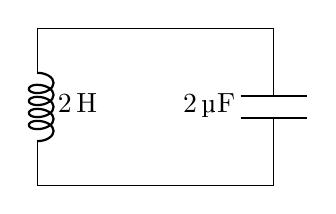
\begin{tikzpicture}[scale=2]
            \draw (0, 0) to (1.5, 0) to [C, l=2<\micro\farad>] (1.5, 1) to (0, 1) to [L, l=2<\henry>] (0, 0);
        \end{tikzpicture}
        \end{center}
        \begin{enumerate}
            \item Write out the DAE.
            \item Show that this circuit is an oscillator.
            \item Find its period.
        \end{enumerate}
    \end{frame}
\end{document}
